\documentclass{beamer}
\usepackage[style=authoryear,backend=biber]{biblatex}
\usepackage[utf8]{vietnam}
\usepackage{subfig}
\usepackage{amssymb}
\usepackage{amsmath}
\usepackage{lmodern}
\usepackage{algorithm}
\usepackage{algorithmic}
\usepackage[math]{iwona}
\usepackage[british]{babel}
\usepackage{graphicx,hyperref,url}
\usetheme{CambridgeUS}
\usecolortheme{orchid}
\usepackage{enumerate}
\usepackage{tikz}
\usepackage{verbatim}
\usepackage{booktabs}
%\usepackage{natbib}
%\bibliographystyle{apalike}
\usetikzlibrary{bayesnet}
\renewcommand{\baselinestretch}{1.2}
\fontsize{16pt}{16pt}\selectfont
\newcommand\Fontvi{\fontsize{6}{7.2}\selectfont}
\setbeamertemplate{itemize/enumerate body begin}{\large}
\setbeamertemplate{itemize/enumerate subbody begin}{\large}

\makeatletter
\def\step{%
   \@ifnextchar[ \@myitem{\@noitemargtrue\@myitem[\@itemlabel:]}}
\def\@myitem[#1]{\item[#1]\mbox{}}
\makeatother
\renewcommand{\baselinestretch}{1.2}
\makeatletter
\renewcommand{\ALG@name}{Thuật toán}
\makeatother
\renewcommand{\algorithmicrequire}{\textbf{Input:}}
\renewcommand{\algorithmicensure}{\textbf{Output:}}

\usepackage{lipsum}

\newenvironment{localsize}[1]
{%
  \clearpage
  \let\orignewcommand\newcommand
  \let\newcommand\renewcommand
  \makeatletter
  \input{bk#1.clo}%
  \makeatother
  \let\newcommand\orignewcommand
}
{%
  \clearpage
}


%\AtBeginSection{\frame{\sectionpage}}
\AtBeginSection[]{\begin{frame}<beamer>\frametitle{}\tableofcontents[currentsection]\end{frame}}

%----------------------------------------------------------------------------------------
%	TITLE PAGE
%----------------------------------------------------------------------------------------

\title[Sentiment Analysis]{Phân tích quan điểm dựa trên mô hình chủ đề.} % The short title appears at the bottom of every slide, the full title is only on the title page

\author{Sinh viên : Vũ Cao Cường} % Your name
\institute[HUST] % Your institution as it will appear on the bottom of every slide, may be shorthand to save space
{
Đại học Bách Khoa Hà Nội \\ % Your institution for the title page
\medskip
\textit{cuongvc93@gmail.com} % Your email address
}
%\date{\today} % Date, can be changed to a custom date
\date{27-05-2016}
\begin{document}
\nocite{*}
\begin{frame}
  \titlepage
\end{frame}
\begin{frame}
  \frametitle{Nội dung}
  \tableofcontents
\end{frame}
\fontsize{14pt}{20pt}\selectfont

% Section titles are shown in at the top of the slides with the current section 
% highlighted. Note that the number of sections determines the size of the top 
% bar, and hence the university name and logo. If you do not add any sections 
% they will not be visible.

%----------------------------------------------------------------------------------------
%	PRESENTATION SLIDES
%----------------------------------------------------------------------------------------

%------------------------------------------------
\section{Phát biểu bài toán}

%------------------------------------------------
\begin{frame}
\frametitle{Bài toán phân tích quan điểm, cảm xúc}
\begin{itemize}
\item Mục tiêu: phân tích quan điểm, cảm xúc, tình cảm.
\item Đối tượng phân tích: sản phẩm, dịch vụ, tổ chức, cá nhân,...
\item Dữ liệu: Reviews, News, Social Network, Forums,..

\end{itemize}
\end{frame}

\begin{frame}
\frametitle{Đối tượng phân tích: dòng xe ô tô}
\begin{center}
\begin{figure}
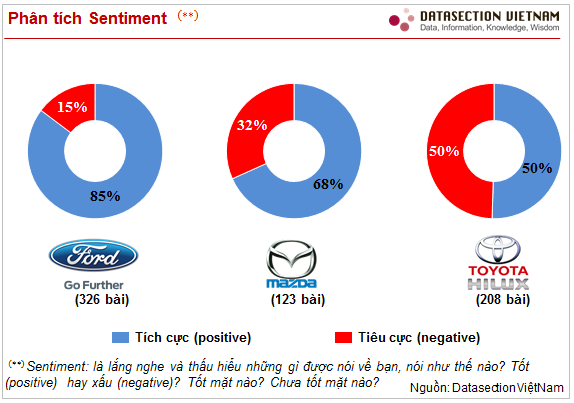
\includegraphics[scale=0.6]{Image/car.png}
\caption*{Đánh giá tỉ lệ quan điểm cho các dòng xe. Nguồn: datasection.com.vn}
\label{labels:1}
\end{figure}
\end{center}
\end{frame}

\begin{frame}
\frametitle{Đối tượng phân tích: các ngân hàng}
\begin{center}
\begin{figure}
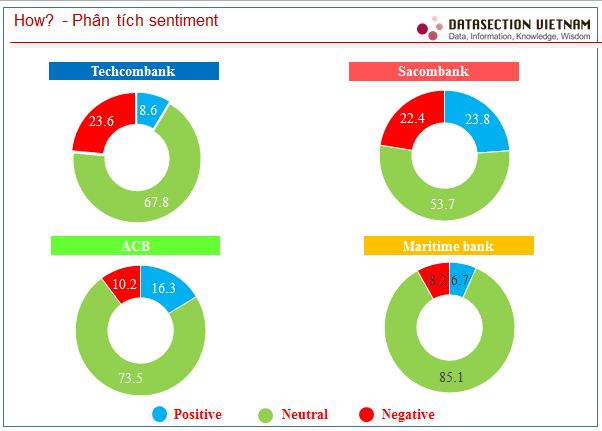
\includegraphics[scale=0.5]{Image/Bank.png}
\caption*{Đánh giá tỉ lệ quan điểm cho các ngân hàng. Nguồn: datasection.com.vn}
\label{labels:1}
\end{figure}
\end{center}
\end{frame}

\begin{frame}
\frametitle{Bài toán phân tích quan điểm, cảm xúc}
Các mức đánh giá:
\begin{itemize}
\item Văn bản, review
\item Câu
\item Khía cạnh (aspect)
\end{itemize}
\end{frame}

\begin{frame}
\frametitle{Đối tượng phân tích: Du lịch Thái Lan}
Mức đánh giá theo văn bản và câu.
\begin{center}
\begin{figure}
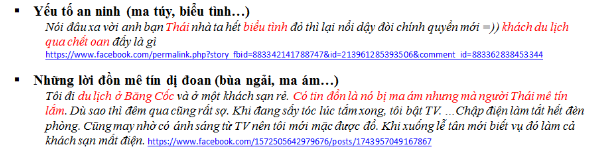
\includegraphics[scale=0.5]{Image/thailan2.png}
\label{labels:1}
\end{figure}
\begin{figure}

\includegraphics[scale=0.5]{Image/thailan3.png}
\caption*{Đánh giá theo văn bản/câu. Nguồn: datasection.com.vn}
\label{labels:1}
\end{figure}
\end{center}
\end{frame}

\begin{frame}
\frametitle{Đối tượng phân tích: Du lịch Thái Lan}
Mức đánh giá theo các khía cạnh.
\begin{center}
\begin{figure}
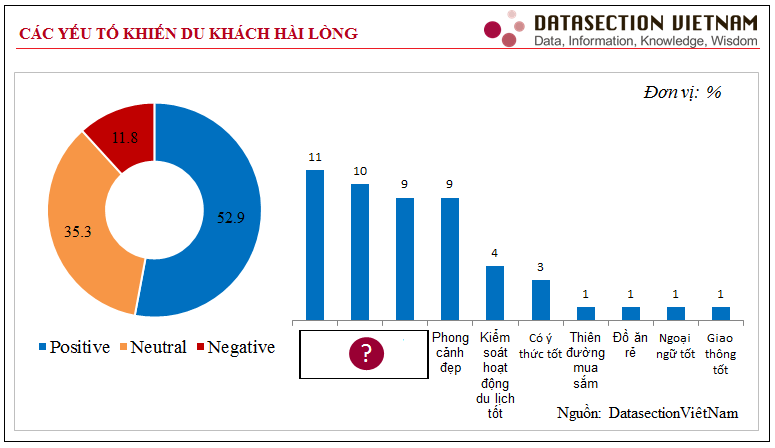
\includegraphics[scale=0.45]{Image/thailan4.png}
\caption*{Đánh giá theo các khía cạnh. Nguồn: datasection.com.vn}
\label{labels:1}
\end{figure}
\end{center}
\end{frame}

\begin{frame}
\frametitle{Đối tượng phân tích: Du lịch Thái Lan}
Mức đánh giá theo các khía cạnh.
\begin{center}
\begin{figure}
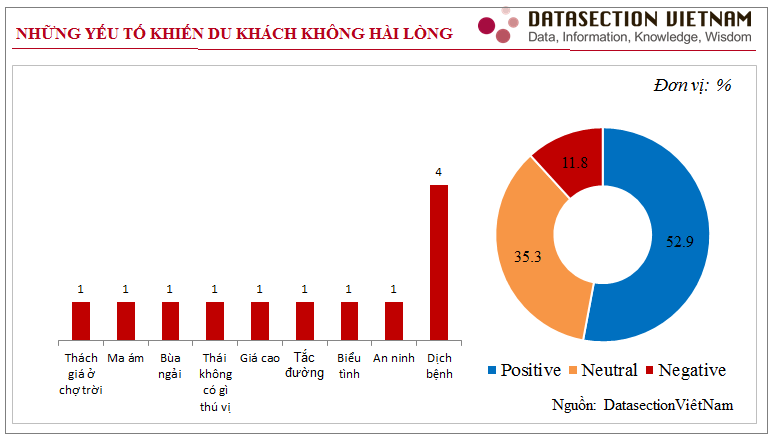
\includegraphics[scale=0.45]{Image/thailan.png}
\caption*{Đánh giá theo các khía cạnh. Nguồn: datasection.com.vn}
\label{labels:1}
\end{figure}
\end{center}
\end{frame}

\begin{frame}
\frametitle{Các phương pháp sử dụng}

\begin{itemize}
\item Sử dụng luật cùng tập từ
\item NLP
\item Học máy phân loại
\item Topic Model
\end{itemize}
\end{frame}

\section{Các mô hình Topic Model đã sử dụng}

%------------------------------------------------
%%%%%%%%%%%%%%%%%%%%%%%%  JST %%%%%%%%%%%%%%%%%%%%%%%%%%%%%%

\begin{frame}
\frametitle{Joint Sentiment and Topic (JST) }
Một văn bản thể hiện nhiều quan điểm và chủ đề khác nhau.
\begin{center}
\begin{figure}
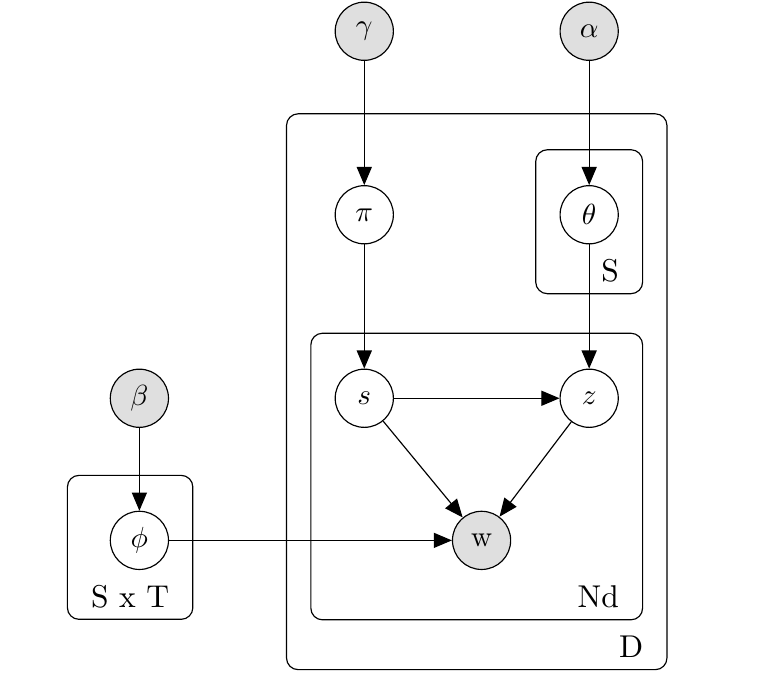
\includegraphics[scale=0.2]{Image/JST.png}
\caption*{Joint Sentiment and Topic model (Lin et al.2009)}
\label{labels:1}
\end{figure}
\end{center}
\end{frame}
%%%%%%%%%%%%%%%%%%%%%%%%  ASUM %%%%%%%%%%%%%%%%%%%%%%%%%%%%%%

\begin{frame}
\frametitle{Aspect and Sentiment Unification Model (ASUM) }
Mỗi câu thể hiện một chủ đề và một quan điểm.
\begin{center}
\begin{figure}
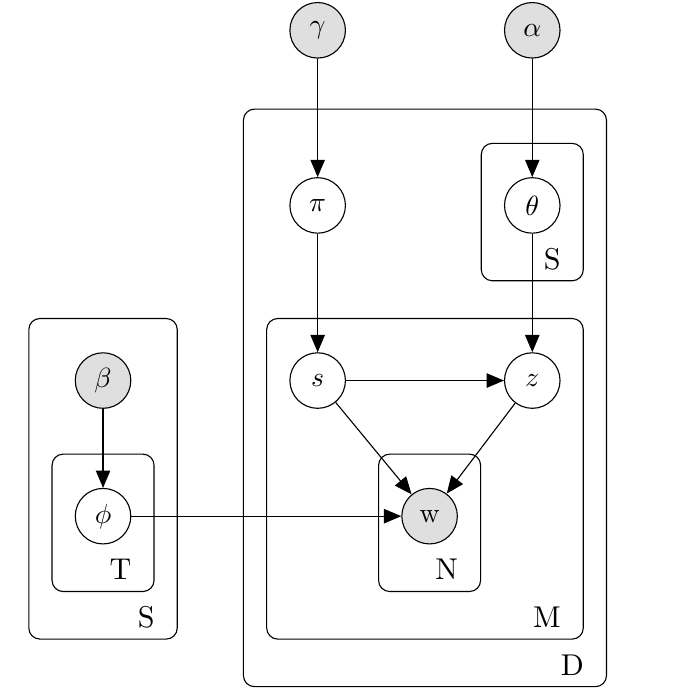
\includegraphics[scale=0.2]{Image/ASUM.png}
\caption*{Aspect and Sentiment Unification Model (Jo et al.2011)}
\label{labels:1}
\end{figure}
\end{center}
\end{frame}
%%%%%%%%%%%%%%%%%%%%%%%%  Nhận xét JST và ASUM %%%%%%%%%%%%%%%%%%%%%%%%%%%%%%

\begin{frame}
\frametitle{Nhận xét mô hình JST và ASUM}
\begin{block}{Nhận xét}
\begin{itemize}
\item Từ có thể có hoặc không thể hiện quan điểm.
\item Từ loại có liên quan tới quyết định là từ quan điểm hay không của từ.
\item Một câu có một quan điểm và một chủ đề là không hợp lí cho văn bản chứa các câu dài.
\end{itemize}
\end{block}
=> mô hình STDP được đề xuất.
\end{frame}

%\section{Sentiment Topic Model with Decomposed Prior}
%%%%%%%%%%%%%%%%%%%%%%%%  STDP %%%%%%%%%%%%%%%%%%%%%%%%%%%%%%

\begin{frame}
\frametitle{Sentiment Topic Model with Decomposed Prior (STDP) }
\begin{center}
\begin{figure}
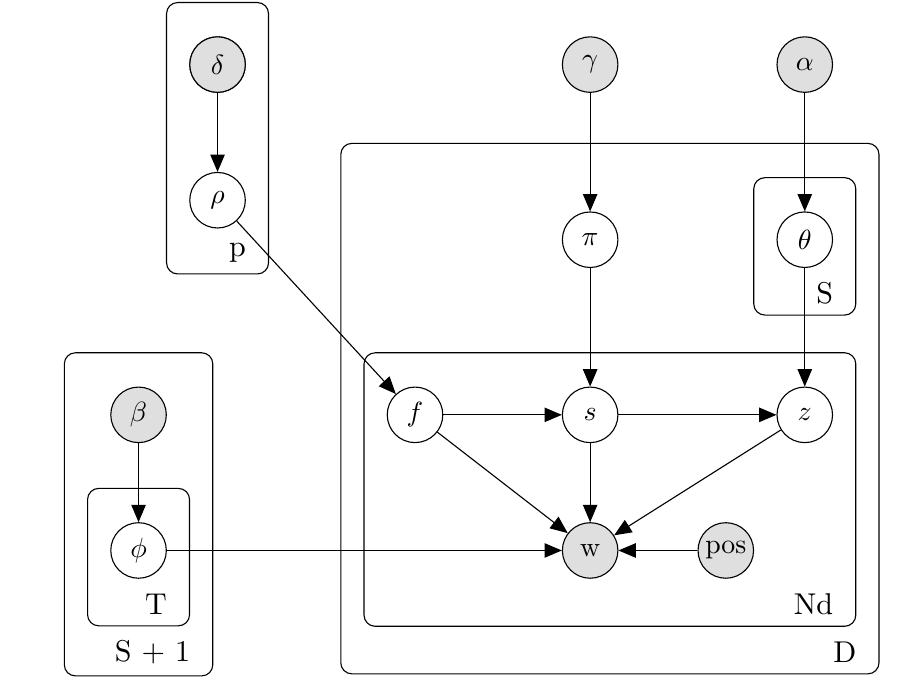
\includegraphics[scale=0.2]{Image/STDP.png}
\caption*{Sentiment Topic Model with Decomposed Prior (Zheng Chen et al.2013)}
\end{figure}
\end{center}
\end{frame}

%%%%%%%%%%%%%%%%%%%%%%%%  Đặc điểm %%%%%%%%%%%%%%%%%%%%%%%%%%%%%%

\begin{frame}
\frametitle{Đặc điểm}
\begin{itemize}
\item Một từ có thể là từ quan điểm hoặc từ thông thường.
\item Từ loại có liên quan tới quyết định là từ quan điểm hay không của từ
\item Một văn bản thể hiện nhiều chủ đề và quan điểm.
\end{itemize}
\end{frame}
%%%%%%%%%%%%%%%%%%%%%%%%  Các nhóm từ loại %%%%%%%%%%%%%%%%%%%%%%%%%%%%%%

\begin{frame}
\frametitle{Các nhóm từ loại và khả năng thể hiện quan điểm }
\begin{table}[htp!]
\caption{Các nhóm từ loại và khả năng thể hiện quan điểm (Zheng Chen et al.2013)}

\centering 
\scalebox{0.8}{
\label{tab:PosTag-Groups}
\begin{tabular}{|c|c|c|c|c|c|}
\hline
 Nhóm từ loại & Kí hiệu & $\delta_1$ \\ \hline
Tính từ & JJ, JJS, JJR & 0.9 \\ \hline 
Trạng từ & RB, RBS, RBR & 0.9\\ \hline
Động từ & VB, VBD, VBG, VBN, VBP, VBZ & 0.7\\ \hline 
Danh từ & NN, NNP, NND, NNPS & 0.9 \\ \hline
Từ khác & các kí hiệu còn lại & 0.1 \\ \hline
\end{tabular}}
\end{table}
$\delta_{1,i}$ là xác suất để từ thuộc nhóm i được đánh giá là từ quan điểm.
\end{frame}

%%%%%%%%%%%%%%%%%%%%%%%%%%%%%%%%%  Mô hình sinh %%%%%%%%%%%%%%%%%%%%%%%%%%%%%%

\begin{frame}[shrink=25]
\frametitle{Quá trình sinh cho văn bản theo STDP}
\begin{center}
       \begin{tabular}{cl}
         \begin{tabular}{c}
             \parbox{0.4\linewidth}{
             	\begin{itemize}
					\item $\phi_{sz} \sim Dir(\beta_{s})$.
					\item $\phi_{(s+1)z} \sim Dir(\beta_{s+1})$.
					\item $\rho_p \sim Beta(\delta_p)$.
					\item Mỗi văn bản d:
					\begin{itemize}
					  \item $\pi_d \sim Dir(\gamma)$.
   					  \item $\theta_{ds} \sim Dir(\alpha)$.
					  \item Mỗi từ trong văn bản:\\
					  	$f \sim Bernouli(\rho_p)$\\
						$f = true$(w là từ quan điểm):
							\begin{itemize}
							 \item $s \sim Mult(\pi_d)$.
							 \item $t \sim Mult(\theta_{ds})$.
							 \item $w \sim Mult(\phi_{ts})$.
							\end{itemize}
						$f = false$ (w từ thông thường):
							\begin{itemize}
							 \item $t \sim Mult(\theta_{d(S+1)})$.
							 \item $w \sim Mult(\phi_{t(S + 1)})$.
							\end{itemize}
					\end{itemize}				
				\end{itemize}
    		}
           \end{tabular}
           & \begin{tabular}{l}
           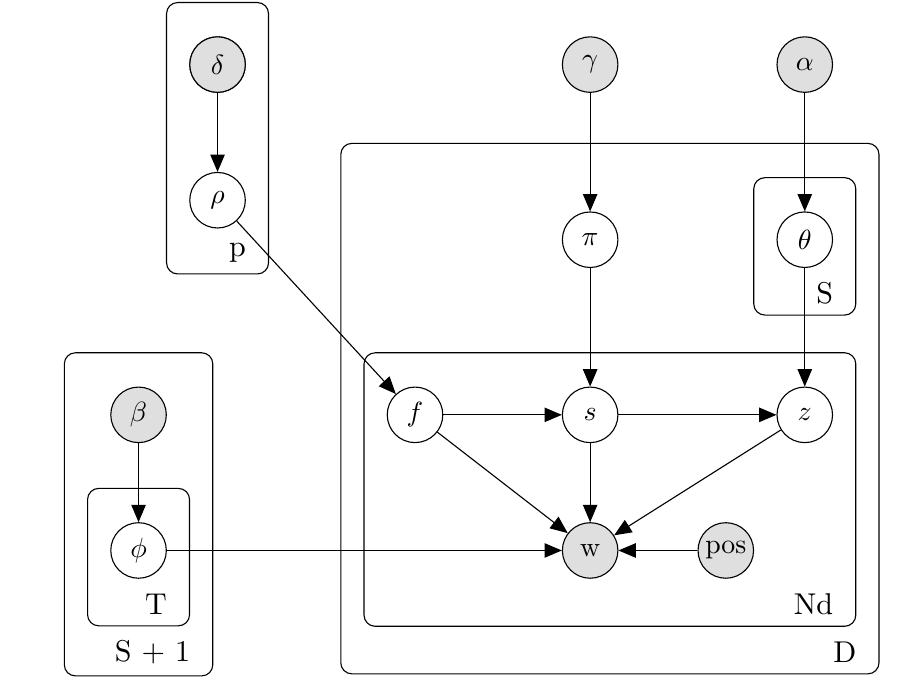
\includegraphics[scale=0.25]{Image/STDP.png}

         \end{tabular}  \\
\end{tabular}\end{center}
\end{frame}
%%%%%%%%%%%%%%%%%%%  Gibbs Sampling - yêu cầu %%%%%%%%%%%%%%%%%%%%%
\begin{frame}
\frametitle{Phương pháp suy diễn Gibbs Sampling}
[Griffiths et al.2002]
\begin{block}{Yêu cầu}
\begin{itemize}
\item Phân phối $p(Z)$ = $p(z_1, z_2,...,z_M)$. \\
\item Cần k mẫu $Z = (z_1, z_2,...,z_M)$ từ $p(Z)$. \\
\end{itemize}
\end{block}
\end{frame}
%%%%%%%%%%%%%%%%%%%%%%%%%%%  Gibbs Sampling %%%%%%%%%%%%%%%%%%%%%

\begin{frame}
\frametitle{Phương pháp suy diễn Gibbs Sampling}
\begin{block}{Giải thuật}
Bước 1: Khởi tạo $z^1 = (z_1, z_2,...,z_M)$\\
Bước 2: Lặp $i = 1,..,k$:
\begin{itemize}
\item $z_1^{(i+1)} \sim p(z_1|z_2^{(i)}, z_3^{(i)},..,z_n^{(i)})$
\\...
\item $z_j^{(i+1)} \sim p(z_j|z_1^{(i+1)}, z_2^{(i+1)},..,z_{j-1}^{(i+1)}, z_{j+1}^{(i)}, z_{j+2}^{(i)},.., z_n^{(i)})$
\\...
\item $z_M^{(i+1)} \sim p(z_M|z_1^{(i+1)}, z_2^{(i+1)},..,z_{(M-1)}^{(i+1)})$
\end{itemize}
\end{block}
\end{frame}

\begin{frame}
\frametitle{Phương pháp suy diễn Gibbs Sampling}
Kết quả:
\begin{itemize}
\item Các mẫu thu được sẽ tạo thành một phân phối gần với phân phối hợp của tất cả các biến.
\item Giá trị kì vọng của các biến có thể tính xấp xỉ bằng cách lấy trung bình giá trị của tất cả các mẫu cho biến đó.
\end{itemize}
\end{frame}
%%%%%%%%%%%%%%%%%%%%%%%%%%%%%%%%%  Learning and Infer %%%%%%%%%%%%%%%%%%%%%%%%%%%%%%

\begin{frame}
\frametitle{Phương pháp học và suy diễn của mô hình}
\begin{block}{Phương pháp suy diễn - Gibbs Sampling}
 \begin{itemize}
 	\item Lấy mẫu $f_i$, $s_i$, $z_i$ cho từ i trong văn bản d
 	\item Tính xấp xỉ $\theta_d$ và $\pi_d$ từ $f_i$, $s_i$, $z_i$ 
 \end{itemize}  
\end{block}

 \begin{block}{Phương pháp học - batch}
 \begin{itemize}
 	\item Lặp trên toàn bộ dữ liệu để tính tham số toàn cục $\phi$
\end{itemize}
\end{block}
\end{frame}

%%%%%%%%%%%%%%%%%%%%%%%%%%%%%%%%%%%%%  Batch Algorithm %%%%%%%%%%%%%%%%%%%%%%%%%%%%%%

\begin{frame}[shrink=22]
\frametitle{}
\begin{center}
       \begin{tabular}{cl}
         \begin{tabular}{c}
             \parbox{0.2\linewidth}{\begin{algorithm}[H]
\begin{algorithmic}
\caption{Thuật toán học Batch cho mô hình STDP}
\label{algo:Batch_STDP}
\REQUIRE{Tham số tiên nghiệm $\beta$, $\alpha$, $\gamma$, $\delta$ và tất cả dữ liệu D văn bản}
\ENSURE{Tính tham số toàn cục $\phi^b$ và $\pi$, $\theta$ cho từng văn bản\\}
Khởi tạo : $\phi^0 \sim Dirichlet(\beta)$\\
\FOR {$i \in 1 ... iter$} 
\FOR {văn bản $d \in D$}
\FOR {từ $i \in d$}
	\STATE{$\forall s \in S, t \in T$, \\ \quad \quad tính $p(f_i=true,s_i=s,t_i=t|w, f_{-i}, s_{-i}, t_{-i})$ }
	
	\STATE{$\forall t \in T$, tính $p(f_i=false,t_i=t|w, f_{-i}, t_{-i})$ }
\ENDFOR\\
\ENDFOR\\
\ENDFOR
\STATE {Tính $pi$}
\STATE {Tính $\theta$}
\STATE {$\phi_{ts}^w = \frac{\beta_s^w + n_{ts}^w}{\sum_{s} (\beta_s^w + n_{ts}^w)}$}
\end{algorithmic}
\end{algorithm}
    		}
           \end{tabular}
           & \begin{tabular}{l}
         \end{tabular}  \\
\end{tabular}\end{center}
\end{frame}

%%%%%%%%%%%%%%%%%%%%%%%%%%%%%%%%%%%%%  MÔ HÌNH SINH %%%%%%%%%%%%%%%%%%%%%%%%%%%%%%%
\begin{comment}
\begin{frame}
\frametitle{Sentiment Topic Model with Decomposed Prior (STDP)}
\begin{center}
       \begin{tabular}{cl}
         \begin{tabular}{c}
             \parbox{0.9\linewidth}{%  change the parbox width as appropiate
             \begin{itemize}
				\item $\phi_{sz} \sim Dir(\beta_{s})$.
				\item $\phi_{(s+1)z} \sim Dir(\beta_{s+1})$.
				\item $\rho_p \sim Beta(\delta_p)$.
				\item Mỗi văn bản d:
				\begin{itemize}{$-$}
					\item $\pi_d \sim Dir(\gamma)$.
					\item $\theta_{ds} \sim Dir(\alpha)$.
					\item Mỗi từ trong văn bản:\\
					$f \sim Bernouli(\rho_p)$\\
					$f = true$(w là từ quan điểm):
					\begin{itemize}
					  \item $s \sim Mult(\pi_d)$.
					  \item $t \sim Mult(\theta_{ds})$.
					  \item $w \sim Mult(\phi_{ts})$.
					\end{itemize}
					$f = false$ (w từ thông thường):
				    \begin{itemize}
					  \item $t \sim Mult(\theta_{d(S+1)})$.
					  \item $w \sim Mult(\phi_{t(S + 1)})$.
					\end{itemize}
				\end{itemize}
			\end{itemize}
    		}
           \end{tabular}
           & \begin{tabular}{l}
           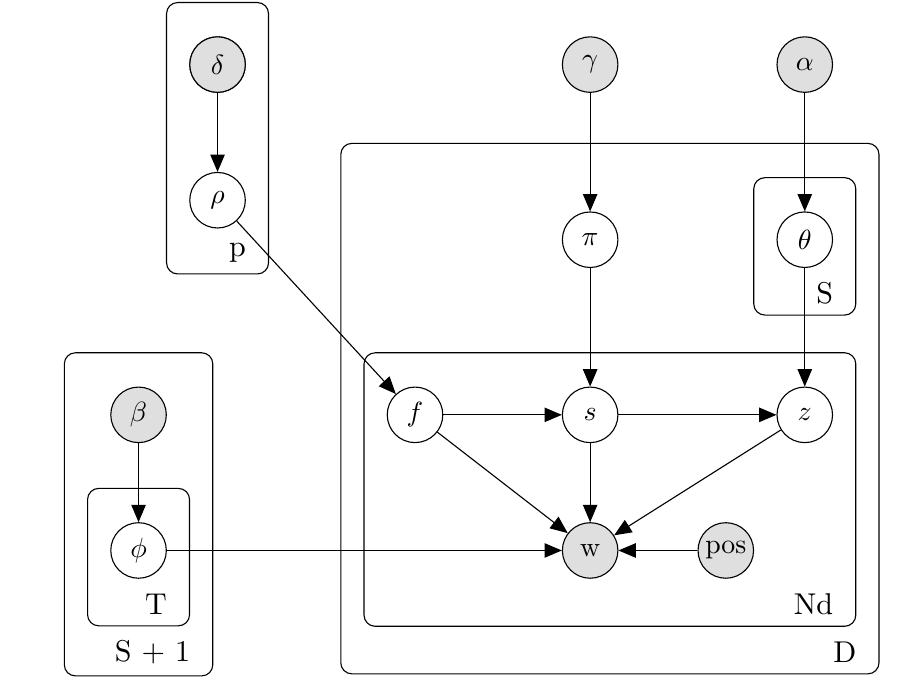
\includegraphics[scale=0.2]{Image/STDP.png}

         \end{tabular}  \\
\end{tabular}\end{center}
\end{frame}
\end{comment}
%%%%%%%%%%%%%%%%%%%%%%%%%%%%%%%%%%% Hạn chế %%%%%%%%%%%%%%%%%%%%%%%%%%%%%%%%%%%

\begin{frame}
\frametitle{Hạn chế của phương pháp học batch}

 \begin{block}{Phương pháp học - batch}
 \begin{itemize}
 	\item Cần lặp đi lặp lại toàn bộ dữ liệu nhiều lần
 	\item Tối ưu trên toàn bộ dữ liệu
\end{itemize}
\end{block}
=> Tốn kém về chi phí bộ nhớ, thời gian và dễ bị rơi vào điểm tối ưu cục bộ.\\      Không hoạt động được trên môi trường dữ liệu vô hạn và tới liên tục.\\
=> cần phương pháp học Online.
\end{frame}


\section{Phương pháp học Online cho mô hình STDP}
%%%%%%%%%%%%%%%%%%%%%%%% Các phương pháp Online-Stream khác %%%%%%%%%%%%%%%%%%%%%%%%%

\begin{frame}
\frametitle{Phương pháp Online}
\begin{block}{batch gradient descent}
\begin{equation}
w_{t+1} = w_t -\gamma_t\frac{1}{L}\sum_{i=1}^{L}\bigtriangledown_wQ(z_n,w_t)
\end{equation}
\end{block}
\begin{block}{online gradient descent (Bottou.1998)}
\begin{equation}
w_{t+1} = w_t - \gamma_t \triangledown_w Q(z_t,w_t)
\end{equation}
Trong đó $z_t$ là một quan sát được chọn ngẫu nhiên trong tập các quan sát.
\end{block}
\end{frame}


%%%%%%%%%%%%%%%%%%%%%%%% Online-stream %%%%%%%%%%%%%%%%%%%%%%%%%
\begin{frame}
\frametitle{Mô hình học online-stream}
\begin{itemize}
\item \textit{Lấy mẫu một minibatch $C_t$ từ tập corpus C}
\item \textit{Ước lượng tham số cục bộ $\pi, \theta$ cho từng văn bản $d \in C_t$ để cực đại hóa $\L_{C_t} = log(p(\pi,\theta|C, \beta, \alpha, \gamma)$)}
\item \textit{Ước lượng tham số toàn cục trung gian $\tilde{\lambda_{st}^t}$ để tối ưu hóa $\L_{C_t}$}
\item \textit{Cập nhật tham số toàn cục}
\end{itemize}
\end{frame}
	

%%%%%%%%%%%%%%%%%%%%%%%% Cập nhật tham số toàn cục %%%%%%%%%%%%%%%%%%%%%%%%%
\begin{frame}
\frametitle{Cập nhật tham số toàn cục}
\begin{block}{stream: SSU (Broderick et al.2013)}
\begin{equation}
\lambda^t \leftarrow \lambda^{t-1} + \tilde{\lambda^t}
\end{equation}
\end{block}
\begin{block}{online: OnlineLDA (Hoffman et al.2010), SVI (Hoffman et al.2013), SSI (Mimno et al.2012)}
\begin{equation}
\lambda^t \leftarrow (1 - \rho_t)\lambda^{t-1} + \rho_t\tilde{\lambda^t}
\end{equation}
\end{block}
$t \rightarrow \infty$ => $\lambda^t$ khó kiểm soát => có thể xảy ra hiện tượng \textbf{overfitting}.
\end{frame}

\begin{frame}
\frametitle{Giải pháp: Regularization (Khoat Than, Tung Doan)}
Chuẩn hóa biến cục bộ trung gian cho các mini-batch:\\
$\tilde{\lambda_{st}^t} \in \Delta_V$, $\Delta_V = \{x \in R^V: x \geq 0,  \sum_{i=1}^{V}x_i=1\}$
\end{frame}

%%%%%%%%%%%%%%%%%%%%%%%% Phương pháp %%%%%%%%%%%%%%%%%%%%%%%%%

\begin{frame}
\frametitle{Mô hình học được đề xuất cho mô hình STDP}
\begin{itemize}
\item \textit{Lấy mẫu một minibatch $C_t$ từ tập corpus C}
\item \textit{Ước lượng tham số cục bộ $\pi, \theta$ cho từng văn bản $d \in C_t$ để cực đại hóa $\L_{C_t} = log(p(\pi,\theta|C, \beta, \alpha, \gamma)$)}
\item \textit{Ước lượng tham số toàn cục trung gian $\tilde{\lambda_{st}^t}$ để tối ưu hóa $\L_{C_t}$ với $\tilde{\lambda_{st}^t} \in \Delta_V$}
\item \textit{Cập nhật $\phi$ : 
 \label{equal:update_phi}
 	\begin{equation}
		\phi^t \leftarrow (1 - \rho_t)\phi^{t-1} + \rho_t\tilde{\lambda^t}
	\end{equation}
}
\end{itemize}
\end{frame}

%%%%%%%%%%%%%%%%%%%%%%%% Gibbs Sampling cho STDP %%%%%%%%%%%%%%%%%%%%%%%%%

\begin{frame}[shrink=25]
\frametitle{Công thức cho suy diễn Gibbs Sampling cho STDP}
Lấy mẫu f, s và z : 
\begin{itemize}
\item Xác suất thể hiện quan điểm
\begin{equation}
\label{equal:sampling_true}
\begin{split}
&p(f_i=true,s_i=s,t_i=t|w, f_{-i}, s_{-i}, t_{-i})  \\ &\sim(\alpha^t + n_{d,s,-i}^t).\phi_{s,t,w_{dn}}.(n_{d,-i}^s+\gamma^s).\frac{n_{p,-i}^{true}+\delta_p^{true}}{n_p^{true} + \delta_p^{true} + n_p^{false} + \delta_p^{false} }
\end{split}
\end{equation}
\item Xác suất không thể hiện quan điểm
\begin{equation}
\label{equal:sampling_false}
\begin{split}
&p(f_i=false,t_i=t|w, f_{-i}, s_{-i}, t_{-i})  \\ &
\sim(\alpha^t + n_{d,s+1,-i}^t).\phi_{s+1,t,w_{dn}}.\frac{n_{p,-i}^{false}+\delta_p^{false}}{n_p^{true} + \delta_p^{true} + n_p^{false} + \delta_p^{false} }
\end{split}
\end{equation}
\end{itemize}
\end{frame}

%%%%%%%%%%%%%%%%%%%%%%%% Tính Pi và Theta %%%%%%%%%%%%%%%%%%%%%%%%%

\begin{frame}[shrink=25]
\frametitle{Công thức tính $\pi$ và $\theta$ cho từng văn bản}
\begin{itemize}
\item Phân phối quan điểm cho văn bản
\begin{equation}
\label{equal:pi}
\pi_{d,s} = \frac{\gamma_s + C_{ds}}{\sum_{s \in S}(\gamma_s+C_{ds}})
\end{equation}
\item Phân phối chủ đề dựa trên quan điểm cho văn bản
\begin{equation}
\label{equal:theta}
\theta_{d,s,t} = \frac{\alpha_t + C_{dst}}{\sum_{t \in T}(\alpha_t+C_{dst}})
\end{equation}
\end{itemize}
\end{frame}

%%%%%%%%%%%%%%%%%%%%%%%% Biến trung gian toàn cục %%%%%%%%%%%%%%%%%%%%%%%%%

\begin{frame}[shrink=25]
\frametitle{Tính biến trung gian toàn cục $\tilde{\lambda}$}
\begin{itemize}
\item Từ thể hiện quan điểm
\begin{equation}
\label{equal:lambda_S}
\tilde{\lambda}_{s,t,j} \sim \ \beta_{s,t,j} + \sum_{d \in C_b} \sum_n \tilde{f}_{n,true}\tilde{s}_{d,n,s}\tilde{z}_{d,n,t}d_{w_{d,n}}^j + k\beta 
\end{equation}
\item Từ không thể hiện quan điểm
\begin{equation}
\label{equal:lambda_S+1}
 \tilde{\lambda}_{s+1,t,j} \sim \beta_{s,t,j} + \sum_{d \in C_b} \sum_n \tilde{f}_{n,false}\tilde{s}_{d,n,(S+1)}\tilde{z}_{d,n,t}d_{w_{d,n}}^j + k\beta 
\end{equation}
\end{itemize}
\end{frame}

%%%%%%%%%%%%%%%%%%%%%%%% Thuật toán học online cho STDP %%%%%%%%%%%%%%%%%%%%%%%%%

\begin{frame}[shrink=25]
\frametitle{Thuật toán học online cho mô hình STDP}
\begin{center}
       \begin{tabular}{cl}
         \begin{tabular}{c}
             \parbox{0.3\linewidth}{
             		\begin{algorithm}[H]
		\begin{algorithmic}
		\caption{Thuật toán học online cho mô hình STDP}
		\label{algo:Online-STDP}
		\REQUIRE{ Tham số tiên nghiệm $\beta$, $\alpha$, $\gamma$, $\delta$, danh sách các minibatch đến liên tục $C^1,C^2,...$}
		\ENSURE{Cập nhật $\phi^b$ sau mỗi minibatch $C^b$\\}
		Khởi tạo : $\phi^0 \sim Dirichlet(\beta)$\\
		\FOR {minibatch $C^b \in C^1,C^2,...$} 

		\STATE {$\rho_t \leftarrow (\tau_0 + t)^{-\kappa}$\\}
		\FOR {văn bản $d \in C^b$}
		\STATE { Khởi tạo $ s_d^0, z_d^0 $ }
		\FOR {từ $i \in d$}
			\STATE{$\forall s \in S, \forall t \in T$, tính $p(f_i=true,s_i=s,t_i=t|w, f_{-i}, s_{-i}, t_{-i})$ } theo \ref{equal:sampling_true}
			\STATE{$\forall t \in T$, tính $p(f_i=false,t_i=t|w, f_{-i}, s_{-i}, t_{-i})$ theo \ref{equal:sampling_false}}
		\ENDFOR\\
		\STATE {Tính $pi$ theo công thức \ref{equal:pi}}
		\STATE {Tính $\theta$ theo công thức \ref{equal:theta}}

		\ENDFOR\\
		\STATE {Tính $\tilde{\lambda}_{stj}$ theo công thức \ref{equal:lambda_S}}
		\STATE {Tính $\tilde{\lambda}_{(s+1)tj}$ theo công thức \ref{equal:lambda_S+1}}
		\STATE {$\tilde{\lambda}_{st} \propto \tilde{\lambda}_{st}$}
		\STATE { $\phi^b \leftarrow (1-\rho_t)\phi^{t-1}+\rho_t\tilde{\lambda}$}
		\ENDFOR
		\end{algorithmic}
		\end{algorithm}
    		}
           \end{tabular}
           & \begin{tabular}{l}
           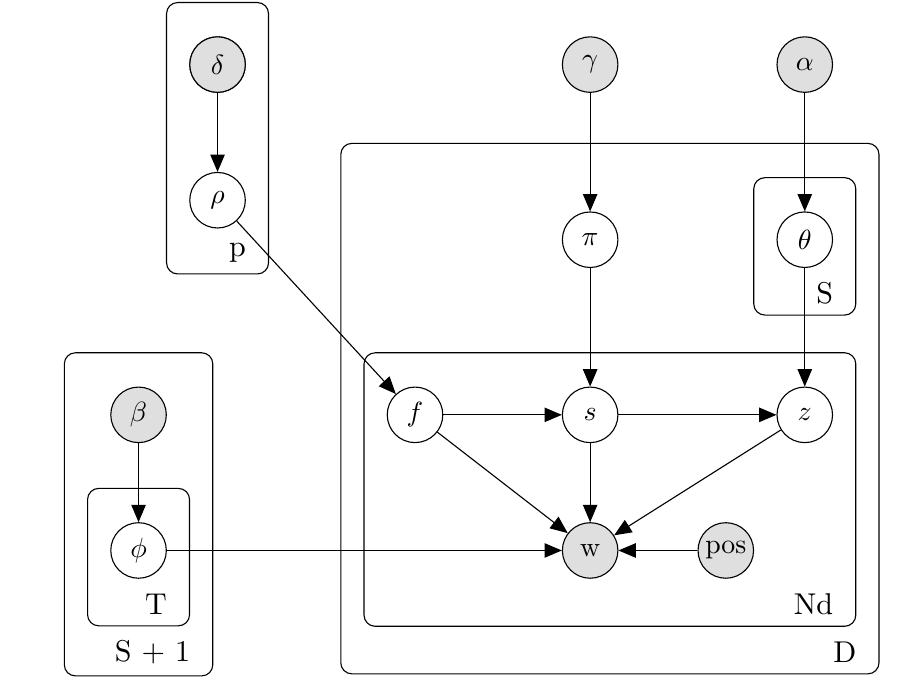
\includegraphics[scale=0.38]{Image/STDP.png}
         \end{tabular}  \\
\end{tabular}
\end{center}
	\end{frame}

%%%%%%%%%%%%%%%%%%%%%%%% Đánh giá tổng quan %%%%%%%%%%%%%%%%%%%%%%%%%

\begin{frame}[shrink=25]
\frametitle{Đánh giá tổng quan}
\begin{block}{So với phương pháp học batch}
\begin{itemize}
\item Có ưu thế rõ ràng về chi phí tính toán và lưu trữ.
\item Có thể có chất lượng phân loại tốt hơn vì có khả năng vượt qua các điểm tối ưu cục bộ.
\item Kì vọng có thể đạt được chất lượng chủ đề tốt hơn.
\end{itemize}
\end{block}
\begin{block}{So với phương pháp học online và stream khác}
\begin{itemize}
\item Có khả năng tránh được overfitting do chuẩn hóa tham số toàn cục trung gian.
\end{itemize}
\end{block}
\end{frame}

\section{Thử nghiệm, đánh giá}
\begin{frame}
\frametitle{Bộ dữ liệu đánh giá}
Đánh giá của người mua hàng trên amazon: 
\begin{itemize}
\item \textbf{baby}  (đồ trẻ em)
\item \textbf{beauty}  (đồ làm đẹp)
\item \textbf{camera and photo}  (máy ảnh, máy quay)
\item \textbf{cellphone and service}  (điện thoại di dộng)
\item \textbf{video}  (phim)
\end{itemize}
\begin{localsize}{10}
  Nguồn:\\ \url{http://www.cs.jhu.edu/~mdredze/datasets/sentiment/}. 
\end{localsize}

\end{frame}

\begin{frame}[shrink=30]
\frametitle{Mô tả dữ liệu sử dụng}
\begin{table}[htp!]
\centering 
\label{tab:dataset_description}
\begin{tabular}{|c|c|p{2cm}|p{2cm}|p{2.2cm}|}
\hline
 Bộ dữ liệu & Số lượng văn bản & Số lượng văn bản tích cực & Số lượng văn bản tiêu cực & Kích thước từ điển \\ \hline
baby & 4256 & 900 & 3356 & 7402\\ \hline 
beauty & 2884 & 493 & 2391 & 7047\\ \hline
camera - photo & 7408 & 1099 & 6309 & 10610\\ \hline 
cellphones - service & 1023 & 384 & 639 & 3861\\ \hline
video & 36180 & 30543 & 5637 & 41140\\ \hline
\end{tabular}
\end{table}
\end{frame}

\begin{frame}
\frametitle{Cách thức thử nghiệm}
\begin{enumerate}
\item Dữ liệu là các review có nhãn tích cực/tiêu cực
\item Sử dụng thông tin là nội dung của các review để dùng trong mô hình
\item Sử dụng kết quả suy diễn quan điểm cho các review ($\pi$) để đánh giá quan điểm cho văn bản.
\end{enumerate}
\end{frame}


\begin{frame}
\frametitle{Các tiêu chí đánh giá}
\begin{enumerate}
\item Chất lượng phân loại quan điểm
\item Tốc độ chạy
\item Chất lượng chủ đề
\item Chất lượng học các từ quan điểm, chủ đề
\end{enumerate}
\end{frame}

\begin{frame}
\frametitle{Chất lượng phân loại quan điểm}
\begin{center}
\begin{table}[t]
	\begin{tabular}{cl}
         \begin{tabular}{c}
            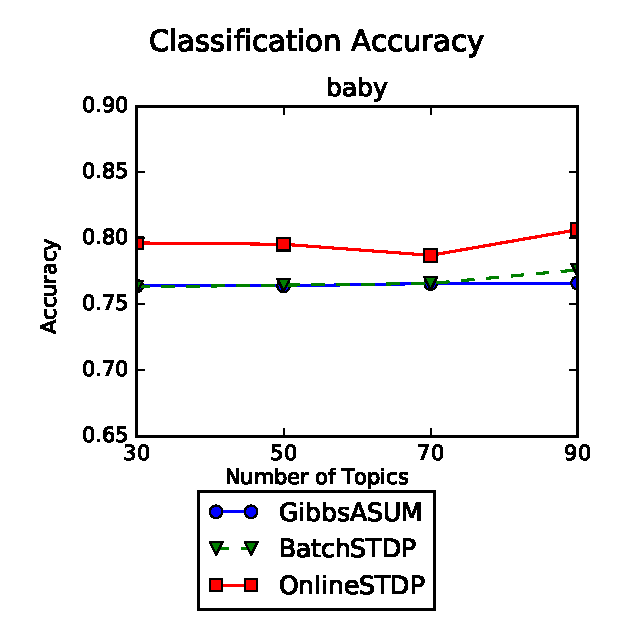
\includegraphics[scale=0.45]{Image/accuracy/baby.eps}
         \end{tabular}
       & \begin{tabular}{l}
            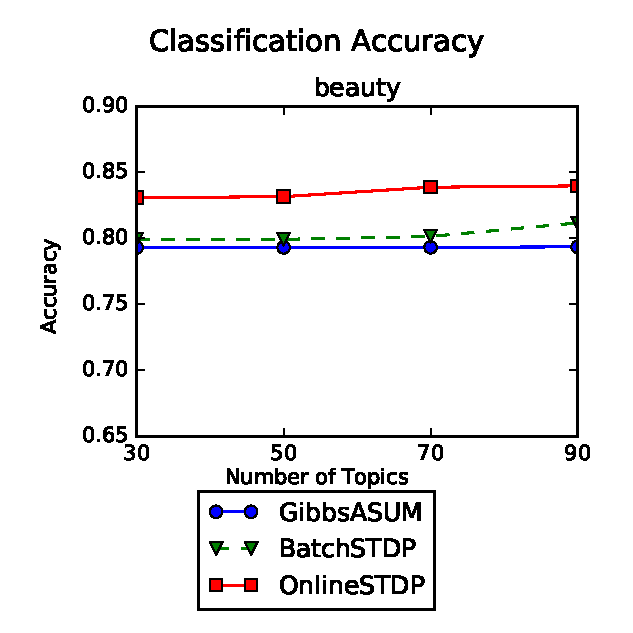
\includegraphics[scale=0.45]{Image/accuracy/beauty.eps}
         \end{tabular}  \\
	\end{tabular}
    \caption*{Kết quả phân loại cho bộ dữ liệu \textit{baby} và \textit{beauty}.}
	
\end{table}
\end{center}
\end{frame}


\begin{frame}
\frametitle{Chất lượng phân loại quan điểm}
\begin{center}
\begin{table}[t]

	\begin{tabular}{cl}
         \begin{tabular}{c}
            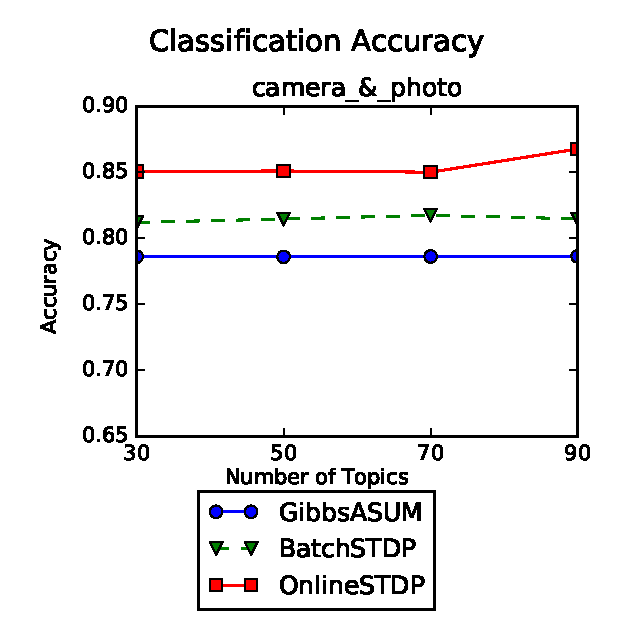
\includegraphics[scale=0.45]{Image/accuracy/camera_photo.eps}
         \end{tabular}
       & \begin{tabular}{l}
            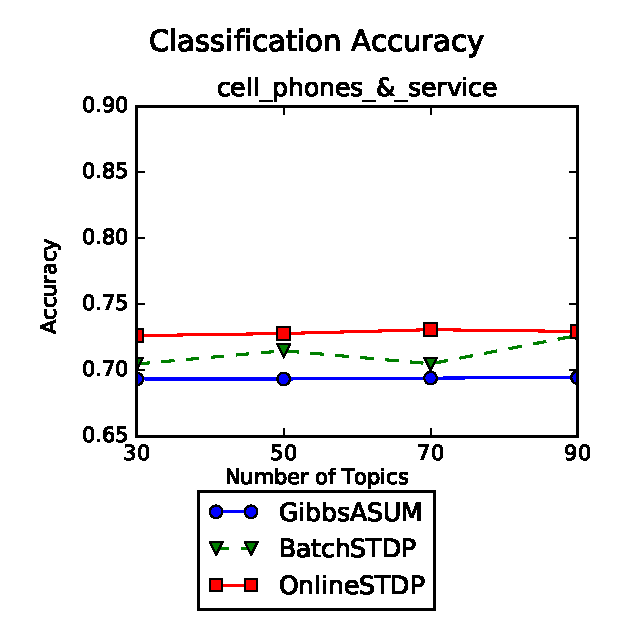
\includegraphics[scale=0.45]{Image/accuracy/cell_phones_service.eps}
         \end{tabular}  \\
	\end{tabular}
    \caption*{Kết quả phân loại bộ dữ liệu \textit{camera and photo} và \textit{cellphone and service}.}
	
\end{table}
\end{center}
\end{frame}

\begin{frame}
\frametitle{Chất lượng phân loại quan điểm}
\begin{center}
\begin{figure}
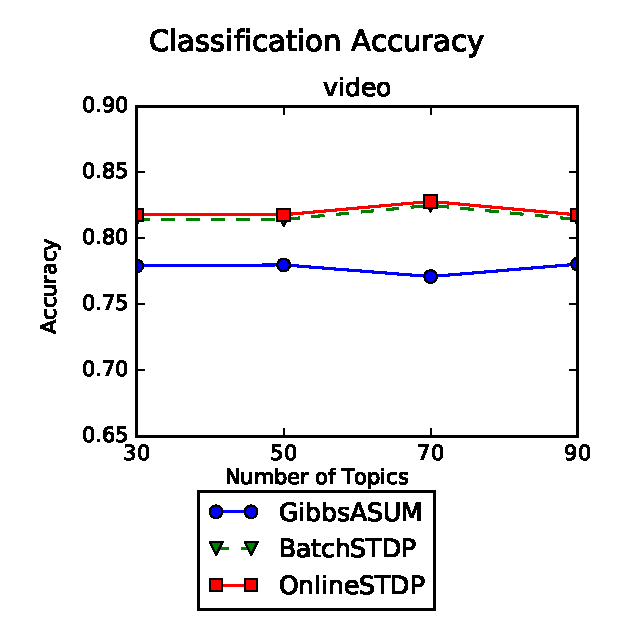
\includegraphics[scale=0.5]{Image/accuracy/video.eps}
\caption*{Kết quả phân loại cho bộ dữ liệu \textit{video}.}
\end{figure}
\end{center}
\end{frame}

\begin{frame}
\frametitle{Chất lượng phân loại quan điểm}
\begin{block}{Nhận xét}
\begin{itemize}
\item Phương pháp học online cho kết quả phân loại quan điểm tốt hơn so với phương pháp học batch.
\item Lí do: phương pháp online có thể vượt qua các điểm tối ưu cục bộ còn phương pháp batch dễ bị rơi vào các điểm tối ưu cục bộ hơn.
\end{itemize}
\end{block}
\end{frame}

\begin{frame}
\frametitle{Thời gian học}
\begin{center}
\begin{figure}
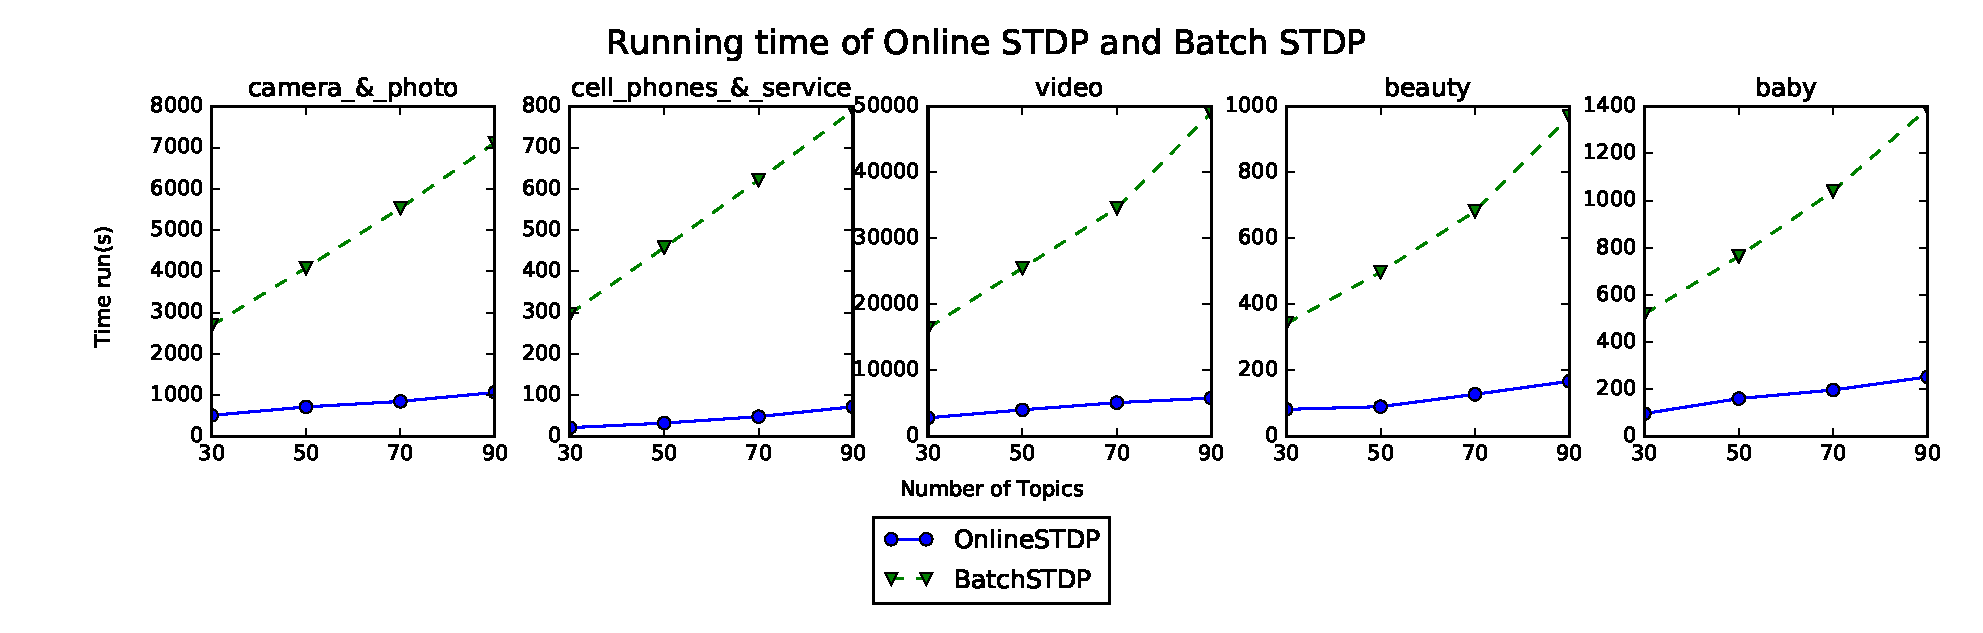
\includegraphics[scale=0.35]{Image/timerun/time_run_vn.eps}
\caption*{Thời gian chạy trên các bộ dữ liệu của BatchSTDP và OnlineSTDP.}
\end{figure}
\end{center}
\end{frame}

\begin{frame}
\frametitle{Thời gian học}
\begin{block}{Nhận xét}
\begin{itemize}
\item Cả 2 phương pháp đều có thời gian chạy là tuyến tính theo số lượng chủ đề.
\item Phương pháp học online cho kết quả về tốc độ chạy là tốt hơn hẳn so với phương pháp batch. 
\item Lí do là phương pháp batch phải lặp đi lặp lại toàn bộ dữ liệu nhiều lần, trong khi online chỉ phải xét một lượt các minibatch.
\end{itemize}
\end{block}
\end{frame}

\begin{frame}[shrink=30]
\frametitle{Chất lượng chủ đề (NPMI)}
\begin{table}[htp!]
\centering 
\caption*{Kết quả so sánh chất lượng chủ đề (NPMI) của phương pháp Batch STDP và Online STDP}
\label{tab:NPMI}
\begin{tabular}{|c|c|c|c|}
\hline
 Bộ dữ liệu & Top & Batch STDP & Online STDP \\ \hline
baby & 10 & 2.22 & 3.12\\ \hline 
beauty & 10 & 2.51 & 2.95\\ \hline
camera and photo & 10 & 4.684 & 5.44\\ \hline 
cellphones and service & 10 & 4.26 & 4.88\\ \hline
video & 10 & 4.82 & 4.928\\ \hline
\end{tabular}
\end{table}
\end{frame}

\begin{frame}
\frametitle{Chất lượng chủ đề (NPMI)}
\begin{block}{Nhận xét}
\begin{itemize}
\item Phương pháp học online có chất lượng chủ đề tốt hơn so với phương pháp học batch.
\end{itemize}
\end{block}
\end{frame}

%%%%%%%%%%%% Khả năng phát hiện chủ đề - quan điểm %%%%%%%%%%%%%%%%%%%%%%
\begin{frame}[shrink=30]
\frametitle{Khả năng phát hiện chủ đề - quan điểm}
\begin{table}[htp!]
\begin{center}
\caption{Các từ có xác suất cao với các chủ đề và quan điểm, bộ dữ liệu Cellphone and Service}
\label{tab:top_word}
\begin{tabular}{llllll}
\toprule
   T0-S0 &    T0-S1 &      T0-S2 &    T1-S0 &      T1-S1 &    T1-S2 \\
\midrule
    good &     dead &       cabl &     good &       burn &  batteri \\
   great &    wrong &      phone &    great &     sucker &   screen \\
    nice &   stupid &    softwar &     fine &       hard &   design \\
  easier &     hard &     driver &  comfort &    useless &    sound \\
 perfect &    cheap &  bluetooth &    smart &        bad &  plastic \\
   worth &    worst &    connect &     free &       poor &     back \\
  strong &      bad &       data &  impress &       loud &   servic \\
    free &   defect &      charg &    worth &        sad &    cover \\
    soft &  useless &     design &     nice &    skeptic &    total \\
 popular &     poor &    batteri &    sleek &  difficult &     treo \\
\bottomrule
\end{tabular}


\end{center}
\end{table}
\end{frame}
%%%%%%%%%%%% Khả năng phát hiện chủ đề - quan điểm %%%%%%%%%%%%%%%%%%%%%%

\begin{frame}
\frametitle{Khả năng phát hiện chủ đề - quan điểm}
\begin{block}{Nhận xét}
\begin{itemize}
\item Có khả năng học ra được các chủ đề trong các quan điểm được nhắc đến.
\item Có khả năng mở rộng tập từ quan điểm và chủ đề, khía cạnh trên một miền dữ liệu.
\end{itemize}
\end{block}
\end{frame}

\section{Tổng kết}
\begin{frame}
\frametitle{Tổng kết}
\begin{block}{Ưu điểm}
\begin{itemize}
\item Tiết kiệm chi phí tính toán và lưu trữ.
\item Thuật toán học online giúp xử lý dữ liệu đến liên tục, không cần biết trước số lượng văn bản.
\item Chuẩn hóa giá trị biến toàn cục trung gian, giảm thiểu được khả năng overfitting..
\item Đạt được kết quả phân loại tốt hơn so với các phương pháp cũ trên cùng mô hình.
\end{itemize}
\end{block}
\end{frame}

\begin{frame}
\frametitle{Tổng kết}
\begin{block}{Nhược điểm}
\begin{itemize}
\item Không có cơ sở lí thuyết để đảm bảo thời gian hội tụ của hàm mục tiêu.
\end{itemize}
\end{block}
\end{frame}

%\begin{frame}[allowframebreaks]
 %       \frametitle{References}
  
 %      \bibliographystyle{amsalpha}
%        \bibliography{reference.bib}
%\end{frame}

\end{document}
